    % IEEE Conference-style Thesis Proposal
    % Compile: pdflatex thesis_proposal.tex && pdflatex thesis_proposal.tex
    \documentclass[conference]{IEEEtran}

    % ---- Packages ----
    \usepackage{cite}
    \usepackage{amsmath,amssymb,amsfonts}
    \usepackage{algorithmic}
    \usepackage{graphicx}
    \usepackage{stfloats}    % Better float placement in two-column mode
    \usepackage{placeins}    % \FloatBarrier to anchor figures near text
    \usepackage{textcomp}
    \usepackage{xcolor}
    \usepackage{booktabs}
    \usepackage{multirow}
    \usepackage{hyperref}
    \usepackage{url}
    \usepackage{tikz}
    \usepackage{pgfplots}
    \pgfplotsset{compat=1.18}
    \usetikzlibrary{shapes.geometric, arrows.meta, positioning, fit, backgrounds, calc, patterns, decorations.pathreplacing}
    \graphicspath{{images/}}

    \renewcommand{\arraystretch}{1.15}

    % TikZ styles
    \tikzset{
        block/.style={rectangle, draw, fill=blue!8, text width=2.2cm, text centered, rounded corners, minimum height=0.8cm, font=\footnotesize},
        blockwide/.style={rectangle, draw, fill=blue!8, text width=3.0cm, text centered, rounded corners, minimum height=0.8cm, font=\footnotesize},
        sensor/.style={rectangle, draw, fill=green!15, text width=1.8cm, text centered, rounded corners, minimum height=0.7cm, font=\footnotesize},
        model/.style={rectangle, draw, fill=orange!20, text width=2.4cm, text centered, rounded corners, minimum height=0.8cm, font=\footnotesize},
        output/.style={rectangle, draw, fill=red!12, text width=2.2cm, text centered, rounded corners, minimum height=0.8cm, font=\footnotesize},
        arrow/.style={-Stealth, thick},
        dashedarrow/.style={-Stealth, thick, dashed},
        layerbox/.style={draw, dashed, rounded corners, inner sep=6pt},
    }

    \begin{document}

    \title{Green-AI: Autonomous Post-Harvest Ripening Control via Distilled Reinforcement Learning on the Edge}

    \author{
    \IEEEauthorblockN{Tristan O. Jadman}
    \IEEEauthorblockA{
    Department of Computer Engineering\\and Mechatronics \\
    \textit{Undergraduate Thesis}}
    \and
    \IEEEauthorblockN{Engr. Francis Jann Alagon}
    \IEEEauthorblockA{
    Department of Computer Engineering\\and Mechatronics \\
    \textit{Thesis Adviser}}
    }

    \maketitle

    % ==============================================================
    \begin{abstract}
    Post-harvest losses account for 20--40\% of tomato production in developing countries, driven by the absence of affordable, intelligent decision-support systems. Existing IoT solutions provide passive monitoring without autonomous action, while cloud-based reinforcement learning (RL) systems require expensive infrastructure and continuous connectivity. This thesis proposes \textit{Edge-RL}, a novel system that deploys a complete RL-based decision pipeline---from visual perception to autonomous ripening control---entirely on a \$33 ESP32-S3 microcontroller. The system extracts a Continuous Chromatic Index ($X \in [0, 1]$, ROYG spectral mapping where $X{=}1$ is Green and $X{=}0$ is Red) from RGB statistics via a MobileNetV2-based feature extractor (INT8, $\sim$300\,KB) and feeds a state vector---including ripening velocity $dX/dt$, remaining time $t_{\text{rem}}$, and colour statistics---to a distilled Deep Q-Network policy (INT8, $\sim$35\,KB) trained via sim-to-real transfer on a physics-based digital twin. Temperature control is implemented as incremental setpoint adjustments ($\pm 1^{\circ}$C), with harvest triggered automatically when the chromatic threshold is reached. An ablation study over three state-space variants (scalar-only, colour statistics, max-pooled spatial features) evaluates feature importance. By leveraging ESP-DL's hardware-optimized inference ($\sim$10$\times$ faster than TFLite Micro), Edge-RL achieves sub-2-second combined inference for spectral feature extraction and control decisions. Hardware-level safety guardrails enforce biological temperature constraints ($12.5$--$35^{\circ}$C) independent of the learned policy. This work presents the first demonstration of a complete sim-to-edge RL pipeline for agricultural post-harvest optimization, offering smallholder farmers an autonomous, connectivity-independent alternative to commercial ripening infrastructure costing \$10,000--\$50,000.
    \end{abstract}

    \begin{IEEEkeywords}
    Edge intelligence, reinforcement learning, post-harvest management, ESP32-S3, sim-to-real transfer, model compression, continuous chromatic index, digital twin
    \end{IEEEkeywords}

    % ==============================================================
    \section{Introduction}
    \label{sec:introduction}

    Global food systems lose approximately 14\% of production between harvest and retail~\cite{fao2019}, with post-harvest losses in developing countries escalating to 20--40\% for perishable crops such as tomatoes~\cite{kader2005}. These losses are not merely agricultural; they represent a \$400 billion annual economic burden and a significant barrier to food security for the estimated 500 million smallholder farming households that produce over 80\% of food consumed in developing economies~\cite{worldbank2020}.

    The tomato supply chain is particularly vulnerable. Ripening is a temperature-dependent, irreversible biochemical process that demands precise timing decisions: harvest too early and fruit quality suffers; harvest too late and shelf life is insufficient for market delivery. Commercial ripening facilities address this with controlled atmosphere storage, real-time monitoring, and expert-driven decision protocols---at costs of \$10,000--\$50,000 per facility~\cite{prasad2018}. For smallholder farmers earning <\$2,000 annually, this infrastructure is entirely inaccessible.

    Three categories of technological solutions have emerged, each with fundamental limitations:

    \textbf{1) Passive IoT monitoring.} Sensor-based systems report environmental conditions (temperature, humidity) but provide no decision support~\cite{ray2017}. They answer ``what is the temperature?'' but not ``when should I harvest given my target delivery date?''

    \textbf{2) Cloud-based agricultural RL.} Reinforcement learning has demonstrated strong results in greenhouse climate control~\cite{chen2022greenhouse} and irrigation scheduling~\cite{yang2020irrigation}. However, these systems require continuous cloud connectivity, incur ongoing operational costs, and introduce latency incompatible with edge deployment in rural settings with intermittent connectivity.

    \textbf{3) Edge classification systems.} Recent work deploys lightweight CNNs on microcontrollers for crop disease detection~\cite{li2021edgeai} and quality grading. These systems classify but do not \textit{decide}---they lack the sequential decision-making capability needed for dynamic optimization over time.

    \textit{Edge-RL bridges all three gaps simultaneously}: it provides autonomous decision-making (not just monitoring), runs entirely at the edge (no cloud dependency), and integrates both perception and sequential optimization (not just classification)---on a \$33 microcontroller.

    \subsection{Research Questions}
    \label{sec:research_questions}

    To address the limitations of existing IoT and Cloud-RL solutions, this study investigates the following questions:

    \begin{enumerate}
        \item[\textbf{RQ1.}] To what extent can Deep Q-Network policies be compressed via knowledge distillation for real-time inference on resource-constrained microcontrollers without significant loss in decision optimality? (Aligned with \textbf{O1})

        \item[\textbf{RQ2.}] How effective is domain randomization within a physics-based digital twin in facilitating zero-shot transfer of harvest timing policies to physical environments with stochastic sensor noise? (Aligned with \textbf{O2})

        \item[\textbf{RQ3.}] Does an autonomous Edge-RL system outperform fixed-schedule heuristic control in balancing post-harvest quality preservation against energy consumption and operational viability? (Aligned with \textbf{O3})
    \end{enumerate}

    \subsection{Research Objectives}

    This study aims to demonstrate:

    \begin{enumerate}
        \item[\textbf{O1.}] \textit{Edge RL feasibility}: A distilled RL policy and a quantized vision model can jointly execute on ESP32-S3 hardware with sub-2-second total inference latency and $\geq$85\% ripeness classification accuracy.

        \item[\textbf{O2.}] \textit{Sim-to-real policy transfer}: An RL harvest timing policy trained entirely in a physics-based digital twin with domain randomization transfers to real sensor data, outperforming fixed-rule baselines.

        \item[\textbf{O3.}] \textit{Operational Efficiency and Viability}: Evaluate the trade-off between harvest quality preservation and energy consumption of the proposed edge intelligence system compared to traditional fixed-schedule methods, demonstrating economic viability for smallholder applications.
    \end{enumerate}

    \subsection{Contributions}

    \begin{enumerate}
        \item The \textbf{first sim-to-edge RL pipeline for post-harvest agriculture} on a sub-\$50 microcontroller, demonstrating that autonomous sequential decision-making is viable at the extreme edge of computing.

        \item A \textbf{physics-based tomato ripening digital twin} implementing a temperature-dependent ODE model with domain randomization, enabling RL policy training without physical crop cycles.

        \item A \textbf{complete open-source reference implementation} of the edge RL pipeline---from training scripts to quantized firmware---enabling reproducibility and extension to other crops.
    \end{enumerate}

    \subsection{Scope and Limitations}
    \label{sec:scope}

    This study focuses on the development and validation of an edge-deployed Reinforcement Learning system for autonomous post-harvest ripening of tomatoes. The scope is defined by the following boundaries:

    \begin{itemize}
        \item \textbf{Crop Focus}: The system is calibrated specifically for tomatoes (\textit{Solanum lycopersicum}) due to their high post-harvest loss rates and climacteric ripening characteristics. While the architecture is portable, model parameters are specific to tomato cultivars.
        \item \textbf{Control Variables}: The agent controls ripening rate solely through temperature modulation using a heater-only actuator system. Humidity is monitored but not actively controlled.
        \item \textbf{Hardware Constraints}: The implementation is strictly limited to the ESP32-S3 microcontroller ($\leq$512KB SRAM) to demonstrate extreme edge feasibility.
        \item \textbf{Environment}: Validations are performed in a controlled chamber environment to isolate variables. Field testing in uncontrolled open-air storage is outside the current scope.
    \end{itemize}

    \noindent \textbf{Limitations}:
    \begin{itemize}
        \item \textbf{Heater-only actuation}: The system can only raise temperature above ambient; it cannot actively cool below $T_{\text{amb}}$. In the Philippine climate ($T_{\text{amb}} \approx 25$--$30^{\circ}$C), this limits the controllable range to $[T_{\text{amb}}, 35^{\circ}$C].
        \item \textbf{Single-fruit Model}: The ODE model and digital twin represent average single-fruit kinetics and do not account for batch-level ethylene interaction effects.
        \item \textbf{Thermal Inertia}: The simulation assumes instantaneous air temperature equilibration, simplifying the thermal lag of the fruit core ($\tau \approx 30$ min).
    \end{itemize}

    \subsection{Conceptual Framework}
    \label{sec:framework}

    The study follows an Input-Process-Output (IPO) model, as illustrated in Fig.~\ref{fig:framework}.

    \begin{figure}[!t]
    \centering
    \resizebox{\columnwidth}{!}{%
    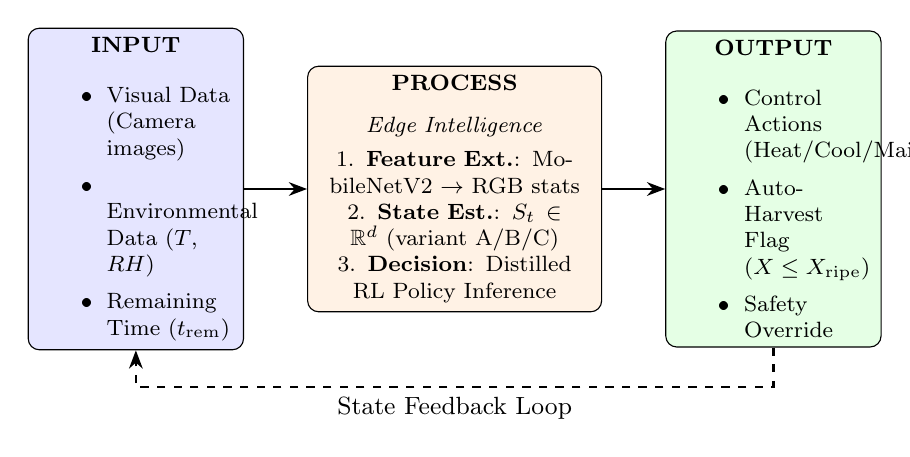
\begin{tikzpicture}[node distance=0.5cm, font=\small]
        % INPUT
        \node[block, fill=blue!10, text width=2.5cm, minimum height=3cm] (input) {
            \textbf{INPUT}\\[0.3cm]
            \begin{itemize}
                \item Visual Data (Camera images)
                \item Environmental Data ($T$, $RH$)
                \item Remaining Time ($t_{\text{rem}}$)
            \end{itemize}
        };

        % PROCESS
        \node[block, fill=orange!10, text width=3.5cm, minimum height=3cm, right=0.8cm of input] (process) {
            \textbf{PROCESS}\\[0.2cm]
            \textit{Edge Intelligence}\\[0.1cm]
            1. \textbf{Feature Ext.}: MobileNetV2 $\to$ RGB stats\\
            2. \textbf{State Est.}: $S_t \in \mathbb{R}^{d}$ (variant A/B/C)\\
            3. \textbf{Decision}: Distilled RL Policy Inference
        };

        % OUTPUT
        \node[block, fill=green!10, text width=2.5cm, minimum height=3cm, right=0.8cm of process] (output) {
            \textbf{OUTPUT}\\[0.3cm]
            \begin{itemize}
                \item Control Actions (Heat/Cool/Maintain)
                \item Auto-Harvest Flag ($X \leq X_{\text{ripe}}$)
                \item Safety Override
            \end{itemize}
        };

        % Arrows
        \draw[arrow] (input) -- (process);
        \draw[arrow] (process) -- (output);
        
        % Feedback
        \draw[arrow, dashed] (output.south) -- ++(0,-0.5) -| (input.south) node[near start, below] {State Feedback Loop};

    \end{tikzpicture}
    }
    \caption{Conceptual Framework of the Edge-RL System. The system processes multi-modal inputs through sequential on-device AI models to produce optimal control actions, forming a closed-loop feedback system with hardware-enforced safety guardrails.}
    \label{fig:framework}
    \end{figure}

    The \textbf{Input} consists of raw visual data captured by the OV2640 camera and environmental readings from the DHT22 sensor. The \textbf{Process} stage involves the core edge intelligence: first, the quantized MobileNetV2 extracts RGB statistics and computes the Continuous Chromatic Index~$X$ (ROYG: $X{=}1$ Green, $X{=}0$ Red); second, this is fused with sensor data, the ripening velocity $\dot{X}$, and the remaining time $t_{\text{rem}}$ into the state vector; third, the distilled RL policy determines the optimal temperature setpoint adjustment. The \textbf{Output} is the incremental actuation command ($\pm \Delta T$), subject to a hard-coded thermal safety override.  Harvest is triggered automatically when $X$ reaches the ripe threshold, creating a feedback loop.

    % ==============================================================
    \FloatBarrier
    \section{Related Work}
    \label{sec:related_work}

    \subsection{Edge AI in Precision Agriculture}

    The deployment of neural networks on microcontrollers---termed \textit{TinyML}~\cite{warden2019tinyml}---has matured rapidly. Banbury et al.~\cite{banbury2021mlperf} established standardized benchmarks for MCU inference, revealing that optimized runtimes can achieve real-time classification on devices with $<$512\,KB SRAM. Lin et al.~\cite{lin2020mcunet} demonstrated that co-designing neural architectures with memory-aware search (MCUNet) achieves ImageNet-level accuracy on ARM Cortex-M class devices, pushing the boundary of what edge AI can accomplish.

    For agricultural deployments specifically, ESP-DL~\cite{espdl2024}---Espressif's native deep learning library for the ESP32-S3---achieves approximately 10$\times$ inference speedup over TensorFlow Lite Micro by exploiting the S3's vector instructions, dual-core scheduling, and automated SRAM/PSRAM memory planning. Prior work has demonstrated plant disease classification~\cite{li2021edgeai}, fruit quality grading~\cite{zhang2021tomato}, and soil monitoring on ESP32 platforms.

    Tomato classification in particular has been extensively studied. Phan et al.~\cite{phan2023tomato} achieved 98--100\% accuracy using CNN architectures (ResNet-50/101) with YOLOv5 for simultaneous detection and classification of ripeness stages. However, these results use server-class GPUs for inference. On-device tomato classification at the microcontroller level remains underexplored, and existing edge systems are exclusively limited to \textit{single-shot classification}---they produce a label at one point in time but do not perform \textit{sequential decision-making} that considers the temporal dynamics of biological processes.

    \subsection{Reinforcement Learning for Agricultural Optimization}

    RL has been applied to greenhouse climate control, where agents learn temperature and humidity setpoint policies that outperform fixed-rule controllers~\cite{chen2022greenhouse}. Hemming et al.~\cite{hemming2020greenhouse} at Wageningen University demonstrated that deep RL (DDPG) can reduce energy consumption by 15--20\% while maintaining crop yield in Dutch greenhouse tomato production. Deep RL approaches---PPO, SAC---have been explored for irrigation scheduling~\cite{yang2020irrigation}, nutrient management, and crop planning.

    Overweg et al.~\cite{overweg2021cropgym} introduced CropGym, a standardized RL environment for crop management that enables reproducible comparison of RL algorithms on agricultural tasks. Tao et al.~\cite{tao2019digital} surveyed the broader digital twin paradigm in industry, establishing the theoretical framework for coupling physical agricultural processes with virtual simulation environments for RL training.

    These works establish RL's capability for agricultural optimization, but all operate with cloud or server-based inference. The computational and connectivity requirements of existing agricultural RL systems limit deployment to well-resourced commercial operations. Our work extends this paradigm by demonstrating that RL policy inference can be performed \textit{directly on the microcontroller} through policy distillation and INT8 quantization. DQN~\cite{mnih2015dqn} is preferred over continuous-action algorithms because the three temperature control commands (maintain, heat, cool) are inherently discrete setpoint adjustments, not points on a continuous scale.

    \subsection{Sim-to-Real Transfer}

    Sim-to-real transfer---training policies entirely in simulation and deploying them in the physical world---is well-established in robotics~\cite{tobin2017sim2real}. Domain randomization, which systematically varies simulator parameters during training, is a key technique for bridging the reality gap~\cite{peng2018simtoreal}. Andrychowicz et al.~\cite{andrychowicz2020matters} demonstrated with OpenAI's Rubik's cube manipulation that automatic domain randomization (ADR) enables zero-shot transfer of complex policies, establishing that sufficiently diverse simulation can substitute for real-world data entirely. Zhao et al.~\cite{zhao2020simtoreal} provide a comprehensive survey of sim-to-real methods, categorizing approaches into domain randomization, domain adaptation, and system identification.

    While extensively studied for robotic manipulation and locomotion, sim-to-real methods have received limited attention in agricultural contexts. Agricultural processes differ fundamentally from robotic tasks: they operate on biological timescales (days rather than seconds), involve irreversible state transitions (ripening cannot be undone), and feature significant natural variability. This thesis applies sim-to-real techniques to post-harvest management, constructing a calibrated digital twin based on established ripening kinetics~\cite{saltveit2005} with domain randomization across cultivar-specific parameters.

    \subsection{Model Compression for Microcontrollers}

    Han et al.~\cite{han2016deep} established the foundational three-stage compression pipeline---pruning, quantization, and Huffman coding---achieving 35--49$\times$ compression on AlexNet and VGGNet without accuracy loss. INT8 post-training quantization alone reduces model size by 4$\times$ from FP32 with minimal accuracy degradation~\cite{jacob2018quantization}. Gholami et al.~\cite{gholami2021survey} provide a comprehensive survey of quantization methods, comparing post-training quantization (PTQ) and quantization-aware training (QAT) across architectures.

    Knowledge distillation~\cite{hinton2015distilling} trains compact student networks to approximate larger teacher networks, enabling further compression. Ruffy and Chahal~\cite{ruffy2019distilling} applied knowledge distillation specifically to RL policies, demonstrating that distilled policies can retain $>$95\% of teacher performance at a fraction of the parameter count---a result central to our edge RL approach. Together, these techniques make it possible to deploy models designed for GPU inference on microcontrollers with $<$512\,KB of SRAM.

    \subsection{Research Gap}

    Table~\ref{tab:gap} summarizes the capabilities of existing approaches against Edge-RL, identifying the gap this thesis addresses.

    \begin{table}[htbp]
    \caption{Capability Comparison: Edge-RL vs. Existing Approaches}
    \label{tab:gap}
    \centering
    \begin{tabular}{@{}p{1.7cm}cccc@{}}
    \toprule
    \textbf{Capability} & \textbf{IoT} & \textbf{Edge AI} & \textbf{Cloud RL} & \textbf{Edge-RL} \\
    \midrule
    Sensing & \checkmark & \checkmark & \checkmark & \checkmark \\
    Classification & & \checkmark & \checkmark & \checkmark \\
    Sequential decisions & & & \checkmark & \checkmark \\
    Offline operation & \checkmark & \checkmark & & \checkmark \\
    Sub-\$50 BOM & \checkmark & \checkmark & & \checkmark \\
    No cloud needed & \checkmark & \checkmark & & \checkmark \\
    \bottomrule
    \end{tabular}
    \vspace{2pt}
    {\scriptsize Edge-RL is the only approach that provides all six capabilities simultaneously.}
    \end{table}

    % ==============================================================
    \FloatBarrier
    \section{System Architecture}
    \label{sec:architecture}

    Edge-RL employs a two-layer architecture: a development host for model training and an ESP32-S3 edge device for real-time inference. The training layer operates offline, producing quantized model artifacts; the edge layer operates autonomously without network connectivity. Fig.~\ref{fig:architecture} illustrates the complete system.

    % ---- Figure: System Architecture (two-column) ----
    \begin{figure*}[htbp]
    \centering
    \resizebox{\textwidth}{!}{%
    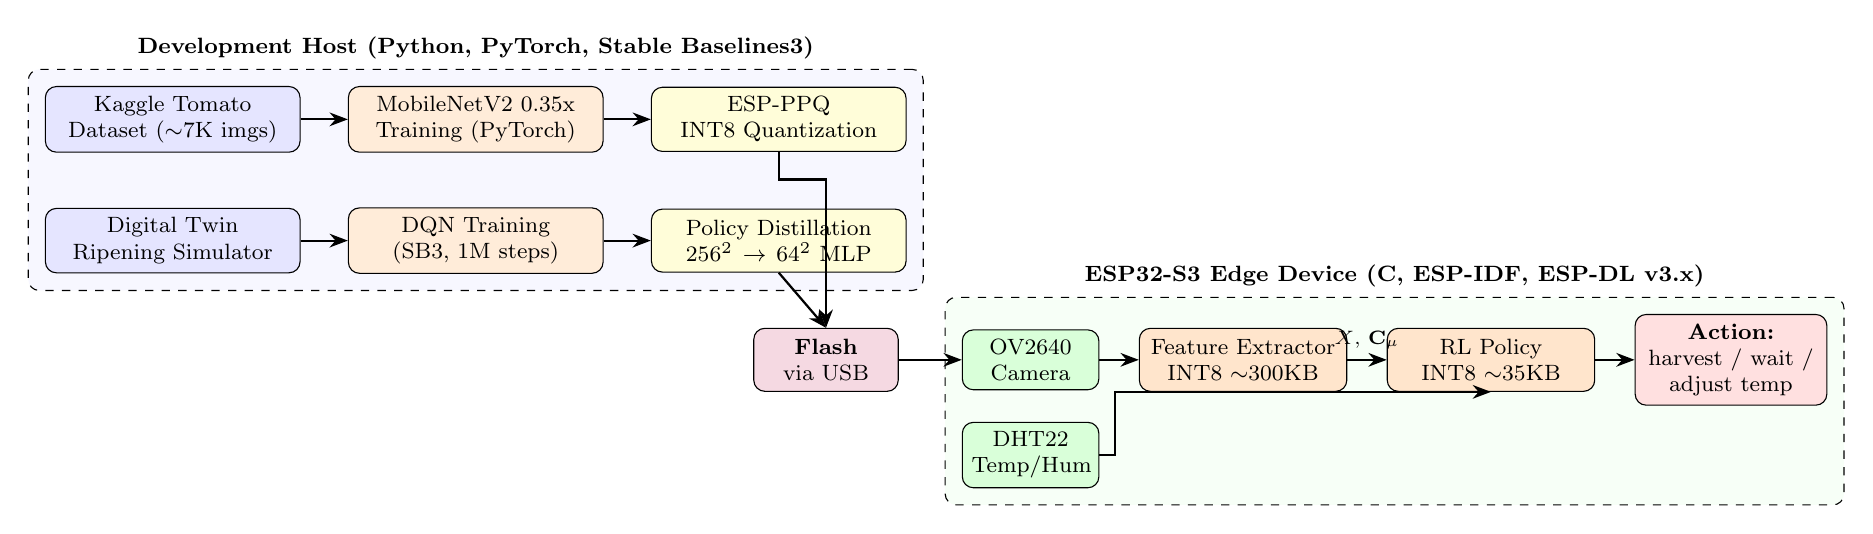
\begin{tikzpicture}[node distance=0.6cm and 0.5cm, font=\footnotesize]

        % === DEVELOPMENT HOST ===
        \node[blockwide, fill=blue!10] (kaggle) {Kaggle Tomato\\Dataset ($\sim$7K imgs)};
        \node[blockwide, fill=orange!15, right=0.6cm of kaggle] (visiontrain) {MobileNetV2 0.35x\\Training (PyTorch)};
        \node[blockwide, fill=yellow!15, right=0.6cm of visiontrain] (quantv) {ESP-PPQ\\INT8 Quantization};

        \node[blockwide, fill=blue!10, below=0.7cm of kaggle] (digtwin) {Digital Twin\\Ripening Simulator};
        \node[blockwide, fill=orange!15, right=0.6cm of digtwin] (dqntrain) {DQN Training\\(SB3, 1M steps)};
        \node[blockwide, fill=yellow!15, right=0.6cm of dqntrain] (distill) {Policy Distillation\\$256^2 \rightarrow 64^2$ MLP};

        \draw[arrow] (kaggle) -- (visiontrain);
        \draw[arrow] (visiontrain) -- (quantv);
        \draw[arrow] (digtwin) -- (dqntrain);
        \draw[arrow] (dqntrain) -- (distill);

        % === FLASH ===
        % Positioned below and between the two rows, centred under quantv/distill
        \node[block, fill=purple!15, text width=1.6cm,
            below=0.7cm of distill, xshift=0.6cm] (flash) {\textbf{Flash}\\via USB};
        % quantv arrow: straight down-right into flash.north
        \draw[arrow] (quantv.south) -- ++(0,-0.35) -| (flash.north);
        % distill arrow: straight down into flash.north (distill is directly above)
        \draw[arrow] (distill.south) -- (flash.north);

        % === ESP32-S3 ===
        \node[sensor, right=0.8cm of flash, fill=green!15, text width=1.5cm] (camera) {OV2640\\Camera};
        \node[model, right=0.5cm of camera] (vmodel) {Feature Extractor\\INT8 $\sim$300KB};
        \node[model, right=0.5cm of vmodel] (rlpol) {RL Policy\\INT8 $\sim$35KB};
        \node[output, right=0.5cm of rlpol] (action) {\textbf{Action:}\\harvest / wait /\\adjust temp};

        \node[sensor, fill=green!15, text width=1.5cm, below=0.4cm of camera] (dht) {DHT22\\Temp/Hum};

        \draw[arrow] (flash) -- (camera);
        \draw[arrow] (camera) -- (vmodel);
        \draw[arrow] (vmodel) -- (rlpol) node[midway, above, font=\scriptsize] {$X$, $\mathbf{C}_\mu$};
        \draw[arrow] (rlpol) -- (action);
        \draw[arrow] (dht.east) -- ++(0.2,0) |- (rlpol.south);

        % Bounding boxes
        \begin{scope}[on background layer]
            \node[layerbox, fill=blue!3, fit=(kaggle)(visiontrain)(quantv)(digtwin)(dqntrain)(distill), label={[font=\footnotesize\bfseries]above:Development Host (Python, PyTorch, Stable Baselines3)}] {};
            \node[layerbox, fill=green!3, fit=(camera)(vmodel)(rlpol)(action)(dht), label={[font=\footnotesize\bfseries]above:ESP32-S3 Edge Device (C, ESP-IDF, ESP-DL v3.x)}] {};
        \end{scope}

    \end{tikzpicture}
    }%
    \caption{Edge-RL system architecture. Two parallel pipelines produce quantized models flashed to the ESP32-S3. The edge device combines camera-based ripeness classification with sensor-informed RL decisions for autonomous harvest timing.}
    \label{fig:architecture}
    \end{figure*}

    \subsection{Hardware Platform}

    The edge device is built around the ESP32-S3-DevKitC-1 (N16R8) with 16\,MB flash, 8\,MB PSRAM, and 512\,KB internal SRAM. Table~\ref{tab:hardware} lists the complete bill of materials at \$33. The wiring topology between the ESP32-S3, camera, sensor, and heater relay is shown in Fig.~\ref{fig:circuit}.

    \begin{table}[htbp]
    \caption{Hardware Bill of Materials}
    \label{tab:hardware}
    \centering
    \begin{tabular}{@{}llr@{}}
    \toprule
    \textbf{Component} & \textbf{Model} & \textbf{Cost} \\
    \midrule
    MCU & ESP32-S3-DevKitC-1 (N16R8) & \$8 \\
    Camera & OV2640 (2MP, 320$\times$240) & \$5 \\
    Sensor & DHT22 ($\pm$0.5°C, $\pm$2\% RH) & \$3 \\
    LED Indicator & WS2812B strip (8 LEDs) & \$2 \\
    Power & USB-C cable + adapter & \$5 \\
    Miscellaneous & Breadboard, wires, enclosure & \$10 \\
    \midrule
    \textbf{Total} & & \textbf{\$33} \\
    \bottomrule
    \end{tabular}
    \end{table}

    \subsection{Memory Architecture}

    Fig.~\ref{fig:memory} shows the memory allocation strategy, which is critical for fitting both models within the ESP32-S3's heterogeneous memory hierarchy. The RL policy ($\sim$35\,KB) resides in fast internal SRAM for low-latency inference, while the larger vision model ($\sim$300\,KB) and its activation buffers are placed in external PSRAM.

    \begin{figure}[!t]
    \centering
    \resizebox{\columnwidth}{!}{%
    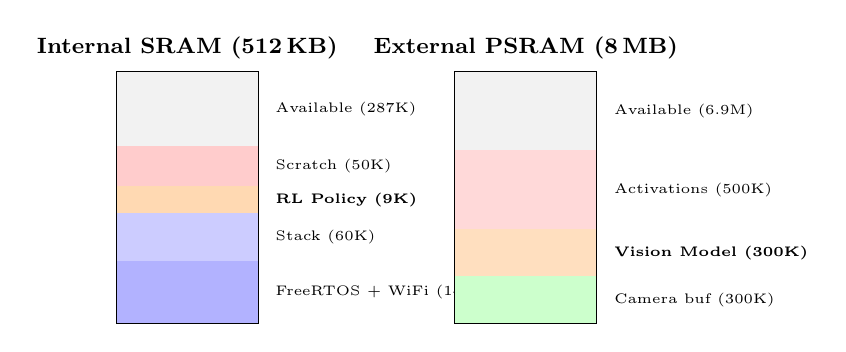
\begin{tikzpicture}[font=\scriptsize]
        % SRAM bar
        \node[font=\footnotesize\bfseries] at (0.9, 3.5) {Internal SRAM (512\,KB)};
        \fill[blue!30] (0,0) rectangle (1.8, 0.80);
        \fill[blue!20] (0,0.80) rectangle (1.8, 1.40);
        \fill[orange!30] (0,1.40) rectangle (1.8, 1.75);
        \fill[red!20] (0,1.75) rectangle (1.8, 2.25);
        \fill[gray!10] (0,2.25) rectangle (1.8, 3.2);
        \draw (0,0) rectangle (1.8, 3.2);
        \node[right, font=\tiny] at (1.9, 0.40) {FreeRTOS + WiFi (140K)};
        \node[right, font=\tiny] at (1.9, 1.10) {Stack (60K)};
        \node[right, font=\tiny] at (1.9, 1.57) {\textbf{RL Policy (9K)}};
        \node[right, font=\tiny] at (1.9, 2.00) {Scratch (50K)};
        \node[right, font=\tiny] at (1.9, 2.72) {Available (287K)};

        % PSRAM bar — shifted left to avoid overflow
        \node[font=\footnotesize\bfseries] at (5.2, 3.5) {External PSRAM (8\,MB)};
        \fill[green!20] (4.3,0) rectangle (6.1, 0.60);
        \fill[orange!25] (4.3,0.60) rectangle (6.1, 1.20);
        \fill[red!15] (4.3,1.20) rectangle (6.1, 2.20);
        \fill[gray!10] (4.3,2.20) rectangle (6.1, 3.2);
        \draw (4.3,0) rectangle (6.1, 3.2);
        \node[right, font=\tiny] at (6.2, 0.30) {Camera buf (300K)};
        \node[right, font=\tiny] at (6.2, 0.90) {\textbf{Vision Model (300K)}};
        \node[right, font=\tiny] at (6.2, 1.70) {Activations (500K)};
        \node[right, font=\tiny] at (6.2, 2.70) {Available (6.9M)};
    \end{tikzpicture}
    }%
    \caption{ESP32-S3 memory allocation. The RL policy resides in fast internal SRAM ($<$1 cycle latency), while the vision model uses external PSRAM. Both models fit well within constraints, leaving significant headroom for firmware and future expansion.}
    \label{fig:memory}
    \end{figure}

    \begin{figure}[!t]
    \centering
    \resizebox{\columnwidth}{!}{%
    \begin{tikzpicture}[node distance=1.5cm, font=\footnotesize]
        % ESP32
        \node[block, fill=green!10, text width=3cm, minimum height=4cm] (esp) {\textbf{ESP32-S3}\\\\(Microcontroller)};

        % Sensors
        \node[sensor, left=1.2cm of esp, yshift=1.2cm] (cam) {OV2640\\Camera};
        \node[sensor, left=1.2cm of esp, yshift=-1.2cm] (dht) {DHT22\\Temp/Hum};

        % Actuators
        \node[output, right=1.2cm of esp, yshift=0cm] (relay) {Relay Module};
        \node[draw, circle, right=0.5cm of relay] (heat) {Heater};

        % Power
        \node[draw, circle, fill=yellow!10, below=1cm of esp] (pwr) {5V PSU};

        % Connections
        \draw[arrow] (cam) -- (esp.west |- cam) node[midway, above, font=\tiny] {CSI};
        \draw[arrow] (dht) -- (esp.west |- dht) node[midway, above, font=\tiny] {GPIO};
        \draw[arrow] (esp.east |- relay) -- (relay) node[midway, above, font=\tiny] {GPIO};
        \draw[arrow] (relay) -- (heat);
        \draw[arrow] (pwr) -- (esp);

    \end{tikzpicture}
    }
    \caption{Circuit Diagram. The ESP32-S3 acts as the central controller, interfacing with the OV2640 camera (CSI), DHT22 sensor (OneWire), and heater relay (GPIO).  No active cooling hardware is present; the ``Cool'' action turns the heater relay OFF, allowing passive thermal dissipation toward ambient.}
    \label{fig:circuit}
    \end{figure}

    % ==============================================================
    \FloatBarrier
    \section{Methodology}
    \label{sec:methodology}

    \subsection{Vision Pipeline: Ripeness Classification}

    \subsubsection{Model Architecture and Rationale}

    We employ MobileNetV2~\cite{sandler2018mobilenetv2} with a width multiplier of 0.35, selected through a three-way trade-off. First, \textit{proven ESP32-S3 compatibility}: Espressif's own benchmarks demonstrate MobileNetV2-INT8 executing in 38\,ms on ESP32-S3 via ESP-DL~\cite{espdl2024}, compared to $>$400\,ms with TFLite Micro. Second, \textit{model size}: the 0.35$\times$ variant produces $\sim$200\,KB of INT8 parameters, comfortably fitting within PSRAM alongside activation buffers. Third, \textit{accuracy}: MobileNetV2's inverted residual blocks with linear bottlenecks preserve representational capacity at reduced widths, achieving competitive accuracy on fine-grained classification tasks despite aggressive compression.

    The standard classifier head is replaced with dropout ($p=0.2$) followed by a linear layer mapping 1280 features to $N$ ripeness classes. The backbone is initialized from ImageNet-pretrained weights and fine-tuned end-to-end. Fig.~\ref{fig:vision_pipeline} illustrates the complete vision pipeline.

    \begin{figure}[!t]
    \centering
    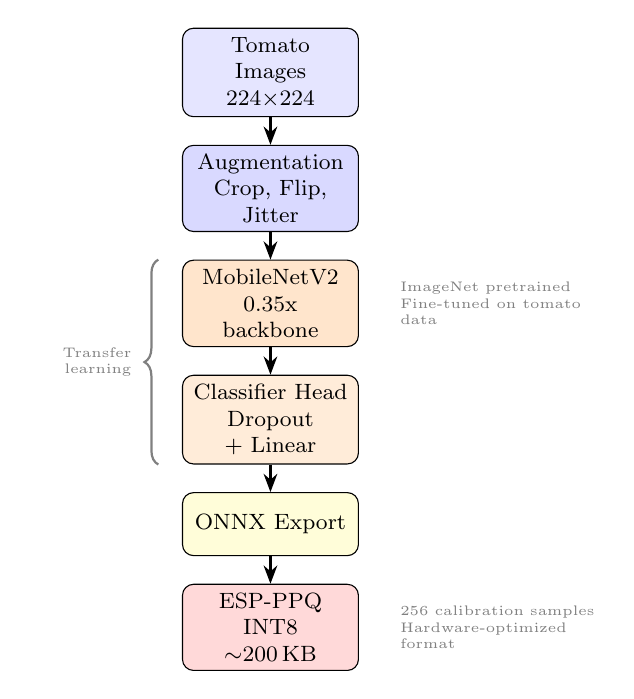
\begin{tikzpicture}[node distance=0.35cm, font=\scriptsize]
        \node[block, fill=blue!10, text width=2.0cm] (data) {Tomato Images\\224$\times$224};
        \node[block, fill=blue!15, text width=2.0cm, below=of data] (aug) {Augmentation\\Crop, Flip, Jitter};
        \node[block, fill=orange!20, text width=2.0cm, below=of aug] (mob) {MobileNetV2\\0.35x backbone};
        \node[block, fill=orange!15, text width=2.0cm, below=of mob] (head) {Classifier Head\\Dropout + Linear};
        \node[block, fill=yellow!15, text width=2.0cm, below=of head] (onnx) {ONNX Export};
        \node[block, fill=red!15, text width=2.0cm, below=of onnx] (quant) {ESP-PPQ INT8\\$\sim$200\,KB};

        \draw[arrow] (data) -- (aug);
        \draw[arrow] (aug) -- (mob);
        \draw[arrow] (mob) -- (head);
        \draw[arrow] (head) -- (onnx);
        \draw[arrow] (onnx) -- (quant);

        % Annotations
        \node[right=0.4cm of mob, text width=2.5cm, font=\tiny, text=gray] {ImageNet pretrained\\Fine-tuned on tomato data};
        \node[right=0.4cm of quant, text width=2.5cm, font=\tiny, text=gray] {256 calibration samples\\Hardware-optimized format};

        % Side arrow for transfer learning
        \draw[decorate, decoration={brace, amplitude=5pt, mirror}, thick, gray] ([xshift=-0.3cm]mob.north west) -- ([xshift=-0.3cm]head.south west) node[midway, left=6pt, font=\tiny, text=gray, text width=1.2cm, align=right] {Transfer\\learning};
    \end{tikzpicture}
    \caption{Vision classification pipeline. Transfer learning from ImageNet provides a strong feature foundation, which is fine-tuned on tomato data and quantized to INT8 via ESP-PPQ for ESP-DL deployment.}
    \label{fig:vision_pipeline}
    \end{figure}

    \subsubsection{Training Procedure}

    Training uses AdamW~\cite{loshchilov2019adamw} with learning rate $\eta = 10^{-3}$, weight decay $\lambda = 10^{-4}$, cosine annealing with 5-epoch linear warmup, and label smoothing ($\epsilon = 0.1$). Data augmentation includes random resized cropping (0.8--1.0$\times$), horizontal flip, $\pm$15° rotation, and color jitter (brightness, contrast, saturation $\pm$0.3; hue $\pm$0.1). The model trains for up to 80 epochs with early stopping (patience 15) on validation accuracy over a 70/15/15 train/val/test split.

    \subsubsection{Quantization via ESP-PPQ}

    The trained model is exported to ONNX and quantized to symmetric INT8 using ESP-PPQ~\cite{espdl2024}. This quantizer is specifically designed for ESP-DL's inference kernels, ensuring that the quantized model fully exploits the ESP32-S3's vector instructions. A calibration set of 256 representative images guides the computation of per-layer scale factors leading to typical accuracy degradation of $<$2\% compared to FP32.

    \subsection{Digital Twin: Physics-Based Ripening Simulator}

    \subsubsection{Continuous Chromatic Index}
    \label{sec:chromatic_index}

    Use of the term ``ripeness'' implies a discrete, subjective agricultural grade.  To ground our system in physically measurable quantities, we define the \textit{Continuous Chromatic Index} $X \in [0, 1]$, a normalized scalar representing the spectral evolution of the tomato surface following the Red-Orange-Yellow-Green (ROYG) spectral mapping:

    \begin{itemize}
        \item $X = 1.0$~: Baseline immature chromatic state (Green, long-wavelength end).
        \item $X = 0.0$~: Target chromatic maturity (Peak Red, short-wavelength end).
    \end{itemize}

    \noindent In an increasing frequency along the visible spectrum, the range proceeds from Red to Green (ROYG). Thus, $X$ maps directly to this spectral ordering: high $X$ corresponds to the green end and low $X$ to the red end.  $X$ is derived from the mean RGB statistics of the tomato ROI by mapping the ROYG spectral shift to a peak-wavelength intensity ratio.  Unlike the 0--5 USDA staging that discretizes a continuous process, $X$ preserves the full gradient of color change, enabling proportional control and fine-grained reward shaping.

    The chromatic index evolves according to a temperature-dependent first-order ODE:
    \begin{equation}
    \frac{dX}{dt} = -k_1 \cdot (T - T_{\text{base}}) \cdot X
    \label{eq:ripening}
    \end{equation}
    \noindent where $k_1$ is the cultivar-specific ripening rate constant, $T$ is the chamber temperature, and $T_{\text{base}} = 12.5^{\circ}$C is the minimum temperature for metabolic activity.  The $X$ multiplicative term creates exponential decay consistent with first-order kinetics: ripening is fastest when $X$ is large (Green) and decelerates as the fruit approaches maturity ($X \to 0$).  The analytical solution is $X(t) = X_0 \cdot \exp(-k_1 (T - T_{\text{base}}) \, t)$, which models the sigmoidal-like kinetics observed in climacteric fruit~\cite{saltveit2005}.

    \subsubsection{State Space Formulation (Restoring the Markov Property)}
    \label{sec:state_space}

    A na\"ive state consisting of the current chromatic index $X_t$ and environmental readings alone violates the Markov property: two tomatoes at identical $X$ but different ripening velocities ($dX/dt$) will follow different future trajectories.  By augmenting the observation vector with the instantaneous velocity $\dot{X}$ and the reference trajectory $X_{\text{ref}}$, the agent observes the system's ``momentum,'' making the future state conditionally independent of the past given the current state.

    We propose three state-space ablation variants of increasing dimensionality to investigate the contribution of visual features:

    \textbf{Option~A} (scalar-only baseline, $\mathbb{R}^{7}$):
    \begin{equation}
    S_t^A = \left[
    X,\; \dot{X},\; X_{\text{ref}},\;
    T,\; H,\; t_e,\; t_{\text{rem}}
    \right]
    \end{equation}

    \textbf{Option~B} (with colour statistics, $\mathbb{R}^{16}$):
    \begin{equation}
    S_t^B = \left[
    X,\; \dot{X},\; X_{\text{ref}},\;
    \mathbf{C}_{\mu},\; \mathbf{C}_{\sigma},\; \mathbf{C}_{\text{mode}},\;
    T,\; H,\; t_e,\; t_{\text{rem}}
    \right]
    \label{eq:state}
    \end{equation}

    \textbf{Option~C} (full feature set, $\mathbb{R}^{20}$):
    \begin{equation}
    S_t^C = S_t^B \;\|\; \mathbf{v}_{\text{mp}}
    \end{equation}

    \noindent where:
    \begin{itemize}
        \item $X \in [0, 1]$: Continuous Chromatic Index (ROYG spectral mapping; $X{=}1$ Green, $X{=}0$ Red).
        \item $\dot{X} = dX/dt$: Instantaneous ripening velocity (finite difference from $t_{-1}$).
        \item $X_{\text{ref}}$: Time-varying reference trajectory computed from the analytical ODE solution at ideal temperature.  Note that $X_{\text{ref}}(t) = \exp(-k_1(T_{\text{ideal}} - T_{\text{base}})\,t)$ is not a constant---it decays over time and serves as a \emph{reference signal} that the agent tracks, analogous to a setpoint in classical control.
        \item $\mathbf{C}_{\mu} \in \mathbb{R}^3$: Mean RGB vector of the tomato ROI (average pooling over full image).
        \item $\mathbf{C}_{\sigma} \in \mathbb{R}^3$: Standard deviation of the RGB vector (texture variance proxy).
        \item $\mathbf{C}_{\text{mode}} \in \mathbb{R}^3$: Per-channel mode (most vivid pixel value), providing the dominant colour present.
        \item $T$, $H$: Current temperature (°C) and relative humidity (\%).
        \item $t_e$: Time elapsed since the start of the episode (days).
        \item $t_{\text{rem}} = t_{\text{tgt}} - t_e$: Remaining time until the target harvest date (days).
        \item $\mathbf{v}_{\text{mp}} \in \mathbb{R}^{4}$: Max-pooled spatial feature vector.  A spatial grid of pixel intensities is divided into 4 regions and the maximum R$-$G difference per region is extracted, analogous to max-pooling in CNNs that identifies the most activated features.
    \end{itemize}

    \noindent The ablation across Options~A, B, and C investigates whether the agent becomes overly dependent on colour/spatial features at the expense of scalar state variables ($X$, $\dot{X}$, $T$, $H$) that carry direct physical meaning.

    \subsubsection{Action Space}

    The action space $\mathcal{A} = \{0, 1, 2\}$ maps to three discrete temperature setpoint commands:
    \begin{itemize}
        \item \textbf{Maintain (0)}: No setpoint change---zero energy cost.
        \item \textbf{Heat (1)}: Increment temperature setpoint by $+\Delta T$ ($= 1^{\circ}$C)---heater relay ON.
        \item \textbf{Cool (2)}: Decrement temperature setpoint by $-\Delta T$ ($= 1^{\circ}$C)---heater relay OFF, passive cooling toward ambient.
    \end{itemize}

    \noindent Temperature actions are \emph{incremental setpoint adjustments} applied to a single-relay heater system.  \textbf{No active cooling hardware} (Peltier, compressor) is present; ``Cool'' physically means turning the heater off and allowing the chamber to passively drift toward the ambient temperature ($T_{\text{amb}} \approx 27^{\circ}$C in the Philippines).  Consequently, the chamber temperature is bounded below by the ambient environment:
    \begin{equation}
    T_{\text{chamber}} \geq T_{\text{amb}}
    \label{eq:ambient_floor}
    \end{equation}
    \noindent This constraint is enforced both in the digital twin (for sim-to-real fidelity) and in the physical hardware (by physics).  The RL agent thus learns to modulate how much \emph{additional} heat to apply above ambient, rather than controlling temperature on a symmetric scale.

    \textbf{Harvest as post-processing.}  Harvest is \emph{not} an explicit action.  Instead, the episode terminates automatically when either (i)~the chromatic index $X$ falls below a ripe threshold ($X \leq 0.15$), or (ii)~the remaining time $t_{\text{rem}} \leq 0$ (deadline reached).  This eliminates the sparsity problem inherent in a terminal harvest action: in each episode, harvest would be called at most once (on success) or never (on failure), making it extremely difficult for the agent to learn its value through standard temporal-difference updates.

    \subsubsection{Reward Function}
    \label{sec:reward}

    The reward function $r_t$ is engineered to enforce safety guardrails while optimizing for rate-appropriate ripening and energy efficiency:

    \begin{equation}
    r_t = r_{\text{track}} + r_{\text{progress}} + c_{\text{safety}} \;(+ \; b_{\text{harvest}} \text{ at termination})
    \label{eq:reward}
    \end{equation}

    \noindent \textbf{1. Rate-Tracking Penalty ($r_{\text{track}}$):} Penalizes deviation between the actual daily ripening rate and the rate required to reach the ripe threshold by the target date:
    \begin{equation}
    r_{\text{track}} = -\lambda \cdot \left|\frac{dX}{dt}_{\text{daily}} - \dot{X}_{\text{desired}}\right|, \quad
    \dot{X}_{\text{desired}} = \frac{X_{\text{ripe}} - X}{\max(t_{\text{rem}},\, \varepsilon)}
    \label{eq:rtrack}
    \end{equation}
    \noindent where $dX/dt_{\text{daily}}$ is the per-step ripening rate converted to daily units, $X_{\text{ripe}} = 0.15$ is the auto-harvest threshold, and $\varepsilon > 0$ prevents singularity as $t_{\text{rem}} \to 0$.  Unit-matching ensures the penalty scale is consistent regardless of the simulation step size.  This naturally balances ``ripen faster'' (when far from target with little time remaining) versus ``slow down'' (when close to target with ample time).

    \noindent \textbf{2. Progress Reward ($r_{\text{progress}}$):} Provides a positive reinforcement signal proportional to actual ripening progress in each step:
    \begin{equation}
    r_{\text{progress}} = \beta \cdot (X_{t-1} - X_t)
    \end{equation}
    \noindent where $\beta$ is a scaling weight.  Since $X$ decreases during ripening (ROYG convention), $(X_{t-1} - X_t) > 0$ whenever the fruit ripens, providing a dense positive reward that prevents the agent from learning a passive ``do-nothing'' strategy.

    \noindent \textbf{3. Capped Progressive Safety Guardrail ($c_{\text{safety}}$):} Safety violations incur a penalty that escalates with \emph{consecutive} boundary violations, capped to prevent catastrophic reward collapse:
    \begin{equation}
    c_{\text{safety}} = \begin{cases}
    -\alpha \cdot \min(n, n_{\text{cap}})^2 & \text{if } T > 35^{\circ}\text{C} \lor T < 12.5^{\circ}\text{C} \\
    0 & \text{otherwise}
    \end{cases}
    \end{equation}
    \noindent where $n$ is the count of consecutive violations, $\alpha = 2.0$, and $n_{\text{cap}} = 5$.  The cap prevents runaway penalties (e.g., $n = 10 \Rightarrow -\alpha \cdot 100$) that would dominate the reward signal and destabilize learning.

    \noindent \textbf{4. Terminal Harvest Bonus ($b_{\text{harvest}}$):} Upon episode termination, a one-time bonus rewards successful ripening:
    \begin{equation}
    b_{\text{harvest}} = \begin{cases}
    b_{\max} \cdot (1 - |t_{\text{rem}}| / t_{\max}) & \text{if auto-harvest } (X \leq 0.15) \\
    0.5 \cdot b_{\max} \cdot (1 - X / 0.5) & \text{if deadline harvest } (t_{\text{rem}} \leq 0)
    \end{cases}
    \end{equation}
    \noindent where $b_{\max} = 10$.  Auto-harvest receives a full bonus scaled by timing accuracy (on-time $\to$ maximum bonus), while deadline harvest receives a partial bonus proportional to how close to ripe the tomato reached.
    \begin{figure}[!t]
    \centering
    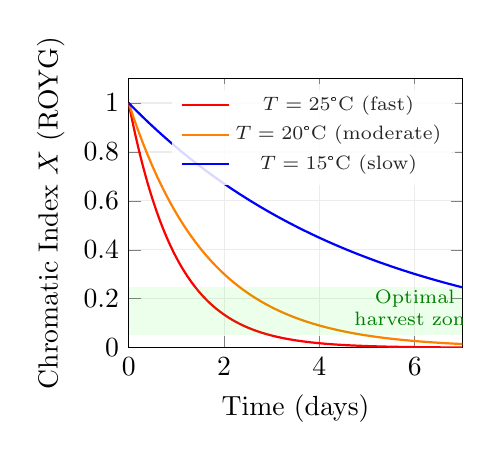
\begin{tikzpicture}
    \begin{axis}[
        width=0.48\textwidth,
        height=5cm,
        xlabel={Time (days)},
        ylabel={Chromatic Index $X$ (ROYG)},
        xmin=0, xmax=7,
        ymin=0, ymax=1.1,
        ytick={0,0.2,0.4,0.6,0.8,1.0},
        legend style={at={(0.98,0.98)}, anchor=north east, font=\scriptsize, draw=none, fill=white, fill opacity=0.85},
        grid=major,
        grid style={gray!15},
        every axis plot/.append style={thick},
    ]
    % T = 25°C (exponential decay from 1)
    \addplot[color=red, smooth, domain=0:7, samples=100]
        {exp(-0.08 * (25 - 12.5) * x)};
    \addlegendentry{$T = 25$\textdegree C (fast)}

    % T = 20°C
    \addplot[color=orange, smooth, domain=0:7, samples=100]
        {exp(-0.08 * (20 - 12.5) * x)};
    \addlegendentry{$T = 20$\textdegree C (moderate)}

    % T = 15°C
    \addplot[color=blue, smooth, domain=0:7, samples=100]
        {exp(-0.08 * (15 - 12.5) * x)};
    \addlegendentry{$T = 15$\textdegree C (slow)}

    % Optimal harvest zone (low X = ripe)
    \fill[green, opacity=0.08] (axis cs:0,0.05) rectangle (axis cs:7,0.25);
    \node[font=\scriptsize, green!50!black] at (axis cs:6.0, 0.20) {Optimal};
    \node[font=\scriptsize, green!50!black] at (axis cs:6.0, 0.12) {harvest zone};

    \end{axis}
    \end{tikzpicture}
    \caption{Simulated chromatic trajectories under ODE model~(\ref{eq:ripening}).  In ROYG convention, $X$ decays from $1.0$ (Green) toward $0.0$ (Red).  Higher temperatures accelerate ripening, compressing the optimal harvest window (green band, $X \in [0.05, 0.25]$). The RL agent must learn to align the trajectory with target delivery schedules.}
    \label{fig:ripening}
    \end{figure}

    \subsubsection{Domain Randomization for Sim-to-Real Transfer}

    To enable policy transfer from simulation to real sensors, we apply domain randomization~\cite{tobin2017sim2real} to five axes of variation per episode: (i)~ripening rate constant $k_1 \sim \mathcal{U}(0.06, 0.10)$, capturing natural variability between tomato cultivars; (ii)~initial chromatic index $X_0 \sim \mathcal{U}(0.6, 1.0)$, representing tomatoes at different starting maturity; (iii)~sensor noise ($\sigma_T = 0.5$\textdegree C, $\sigma_H = 2.0$\%), matching DHT22 specifications; (iv)~temperature drift ($\pm$0.5\textdegree C sinusoidal variation), simulating imperfect environmental control; and (v)~ambient temperature $T_{\text{amb}} \sim \mathcal{N}(27, 2)$\textdegree C, reflecting typical Philippine diurnal variation.  The ambient floor constraint (Eq.~\ref{eq:ambient_floor}) is enforced during training so the policy never learns to rely on active cooling. Fig.~\ref{fig:domain_rand} shows the effect of domain randomization on trajectory diversity.

    \begin{figure}[!t]
    \centering
    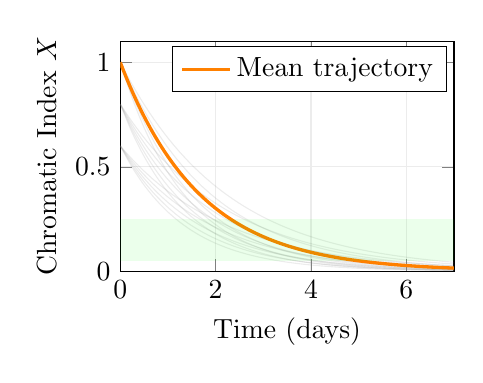
\begin{tikzpicture}
    \begin{axis}[
        width=0.48\textwidth,
        height=4.5cm,
        xlabel={Time (days)},
        ylabel={Chromatic Index $X$},
        xmin=0, xmax=7,
        ymin=0, ymax=1.1,
        grid=major,
        grid style={gray!15},
    ]

    % Envelope: randomized trajectories (light gray)
    \foreach \k in {0.06,0.07,0.08,0.09,0.10} {
        \foreach \rinit in {0.6, 0.8, 1.0} {
            \addplot[gray, opacity=0.15, smooth, domain=0:7, samples=30, forget plot]
                {\rinit * exp(-\k * (20 - 12.5) * x)};
        }
    }

    % Mean trajectory
    \addplot[orange, very thick, smooth, domain=0:7, samples=100]
        {exp(-0.08 * (20 - 12.5) * x)};
    \addlegendentry{Mean trajectory}

    % Harvest zone (low X = ripe)
    \fill[green, opacity=0.08] (axis cs:0,0.05) rectangle (axis cs:7,0.25);

    \end{axis}
    \end{tikzpicture}
    \caption{Domain randomization produces diverse training trajectories (gray envelope), forcing the RL agent to develop robust policies that generalize across varying cultivars, initial conditions, and sensor noise---critical for sim-to-real transfer.}
    \label{fig:domain_rand}
    \end{figure}

    \subsection{Reinforcement Learning Pipeline}

    The ripening control problem is formulated as a Markov Decision Process.  The state space $\mathcal{S} \subset \mathbb{R}^{d}$ (where $d \in \{7, 16, 20\}$ depending on the ablation variant), action space $\mathcal{A}$, and reward function $r_t$ are defined in Section~\ref{sec:state_space} and~\ref{sec:reward}; they are not repeated here.  Fig.~\ref{fig:reward} provides a visual summary of the reward structure.

    \begin{figure}[!t]
    \centering
    \resizebox{\columnwidth}{!}{%
    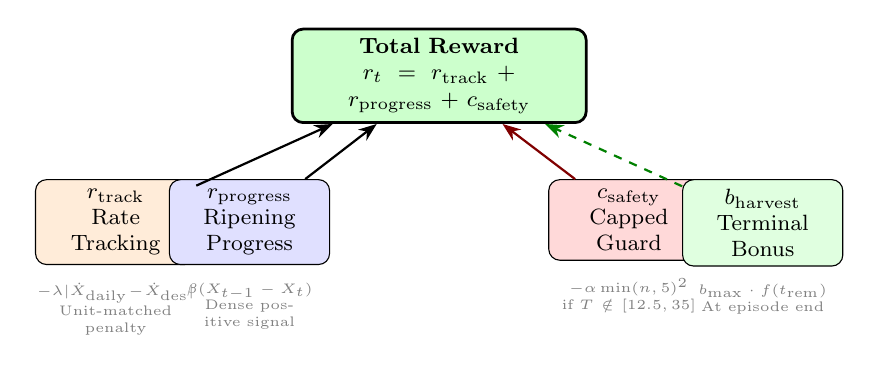
\begin{tikzpicture}[font=\scriptsize, node distance=0.3cm]
        % Total reward
        \node[block, fill=green!20, text width=3.5cm, minimum height=0.9cm, line width=1pt] (total) {\textbf{Total Reward}\\$r_t = r_{\text{track}} + r_{\text{progress}} + c_{\text{safety}}$};

        % Four components
        \node[block, fill=orange!15, text width=1.8cm, below left=0.7cm and 1.2cm of total] (rtrack) {$r_{\text{track}}$\\Rate Tracking};
        \node[block, fill=blue!12, text width=1.8cm, below left=0.7cm and -0.5cm of total] (rprog) {$r_{\text{progress}}$\\Ripening Progress};
        \node[block, fill=red!15, text width=1.8cm, below right=0.7cm and -0.5cm of total] (csafe) {$c_{\text{safety}}$\\Capped Guard};
        \node[block, fill=green!12, text width=1.8cm, below right=0.7cm and 1.2cm of total] (bharvest) {$b_{\text{harvest}}$\\Terminal Bonus};

        \draw[arrow] (rtrack) -- (total);
        \draw[arrow] (rprog) -- (total);
        \draw[arrow, red!50!black] (csafe) -- (total);
        \draw[arrow, dashed, green!50!black] (bharvest) -- (total);

        % Descriptions
        \node[below=0.1cm of rtrack, text width=2.0cm, align=center, font=\tiny, text=gray] {$-\lambda|\dot{X}_{\text{daily}} - \dot{X}_{\text{des}}|$\\Unit-matched penalty};
        \node[below=0.1cm of rprog, text width=2.0cm, align=center, font=\tiny, text=gray] {$\beta(X_{t-1} - X_t)$\\Dense positive signal};
        \node[below=0.1cm of csafe, text width=2.0cm, align=center, font=\tiny, text=gray] {$-\alpha \min(n,5)^2$\\if $T \notin [12.5, 35]$};
        \node[below=0.1cm of bharvest, text width=2.0cm, align=center, font=\tiny, text=gray] {$b_{\max} \cdot f(t_{\text{rem}})$\\At episode end};
    \end{tikzpicture}
    }%
    \caption{Four-component reward structure.  The agent tracks the desired ripening rate ($r_{\text{track}}$), receives dense positive reward for ripening progress ($r_{\text{progress}}$), is penalized for thermal boundary violations with a capped progressive guard ($c_{\text{safety}}$), and receives a terminal harvest bonus scaled by timing accuracy ($b_{\text{harvest}}$, dashed).}
    \label{fig:reward}
    \end{figure}

    \subsubsection{DQN Training}

    We train a Deep Q-Network (DQN)~\cite{mnih2015dqn} using Stable Baselines3~\cite{raffin2021sb3} with a two-layer MLP (256$\times$256 hidden units). Training proceeds for 1M timesteps across 4 parallel environments with the following hyperparameters: $\epsilon$-greedy exploration with linear decay from 1.0 to 0.05 over 30\% of training, target network update interval of 1,000 steps, learning rate $3 \times 10^{-4}$, discount factor $\gamma = 0.99$, replay buffer size $10^5$, and batch size 256. DQN is preferred over continuous-action algorithms (SAC, PPO) because the action space is inherently discrete---the three temperature setpoint commands represent qualitatively different interventions. The compact 3-action space (maintain, heat~$+\Delta T$, cool~$-\Delta T$) also accelerates exploration compared to larger action spaces.

    \subsubsection{Policy Distillation for Edge Deployment}

    The trained DQN teacher (256$\times$256 MLP, $\sim$270\,KB FP32) far exceeds the ESP32-S3's SRAM budget. We distill it into a compact student policy (64$\times$64 MLP) via supervised learning on $10^5$ teacher-generated state-action pairs. The student is trained via cross-entropy loss for 100 epochs with cosine LR decay, then quantized to INT8 ($\sim$35\,KB). Fig.~\ref{fig:distillation} illustrates the compression pipeline.

    \begin{figure}[!t]
    \centering
    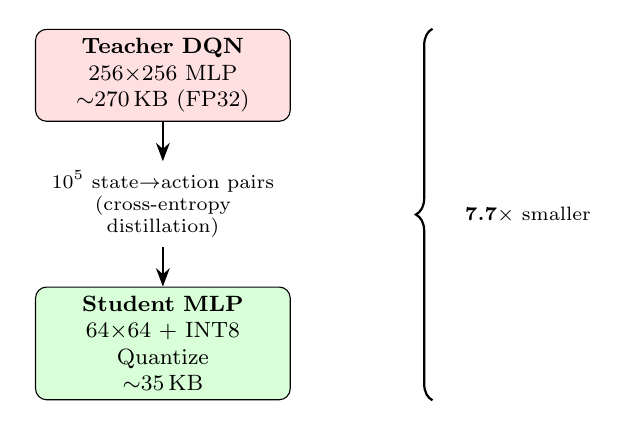
\begin{tikzpicture}[node distance=0.4cm, font=\footnotesize]
        \node[block, fill=red!12, text width=3.0cm, minimum height=1.0cm] (teacher) {\textbf{Teacher DQN}\\256$\times$256 MLP\\$\sim$270\,KB (FP32)};

        \node[below=0.5cm of teacher, text width=3.2cm, align=center, font=\scriptsize] (rollout) {$10^5$ state$\rightarrow$action pairs\\(cross-entropy distillation)};
        \draw[arrow] (teacher) -- (rollout);

        \node[block, fill=green!15, text width=3.0cm, minimum height=1.0cm, below=0.5cm of rollout] (student) {\textbf{Student MLP}\\64$\times$64 + INT8 Quantize\\$\sim$35\,KB};
        \draw[arrow] (rollout) -- (student);

        % Compression factor — reduced offset to stay in column
        \draw[decorate, decoration={brace, amplitude=6pt, mirror}, thick] ([xshift=1.8cm]teacher.north east) -- ([xshift=1.8cm]student.south east) node[midway, right=8pt, font=\scriptsize] {\textbf{7.7$\times$} smaller};
    \end{tikzpicture}
    \caption{Policy distillation and quantization pipeline. Cross-entropy distillation preserves $>$95\% of teacher performance while achieving 7.7$\times$ compression, making the policy deployable in ESP32-S3 internal SRAM.}
    \label{fig:distillation}
    \end{figure}

    \subsection{Hardware Integration \& Actuation Circuitry}

    Transitioning from simulation to physical deployment requires robust handling of high-voltage loads and thermal management. The hardware interface design focuses on isolation and stability:

    \subsubsection{Relay Logic \& Actuation}
    The ESP32-S3's 3.3V GPIOs cannot directly drive the 12V/60W heating element. We utilize a dual-channel 5V relay module with optocoupler isolation to interface the MCU with the high-power load. The relay provides galvanic isolation, protecting the sensitive microcontroller from back-EMF spikes generated during heater switching. A flyback diode is installed across the heater terminals to further suppress inductive kickback.  The three RL actions map directly to a single relay channel: \textbf{Heat}~($a{=}1$) sets the relay HIGH (heater ON); \textbf{Cool}~($a{=}2$) sets the relay LOW (heater OFF, passive cooling toward ambient); \textbf{Maintain}~($a{=}0$) leaves the relay in its current state.  No active cooling hardware (Peltier module or compressor) is included; the chamber temperature cannot be driven below the ambient environment.

    \subsubsection{Power Management}
    A dual-rail power supply unit (PSU) manages energy distribution. A 12V/5A rail powers the heating element, while a buck converter steps this down to a stable 5V/2A rail for the ESP32-S3, sensors, and internal circulation fan. This separation prevents voltage sags on the 12V line (during heater startup) from causing brownouts on the logic rail, ensuring reliable continuous operation.

    \subsubsection{Thermal Enclosure Design}
    The ripening chamber is constructed from 25mm extruded polystyrene foam (XPS) to minimize thermal leakage. To ensure the single-point DHT22 sensor provides a representative measurement of the entire chamber volume, a 12V circulation fan runs continuously to homogenize the air temperature, preventing the formation of hot spots near the heating element or cold pockets in corners.

    \subsection{Edge Inference Architecture}

    The ESP32-S3 firmware is developed using ESP-IDF v5.1+ with FreeRTOS, implementing five concurrent tasks distributed across two CPU cores (Fig.~\ref{fig:freertos}). Critical design decisions include: (i)~pinning vision inference to Core~1 to avoid competing with sensor and communications tasks on Core~0; (ii)~placing the RL policy in internal SRAM for $<$1-cycle memory access latency; and (iii)~triggering inference on-demand (when a new image is captured) rather than polling, to minimize power consumption.

    The firmware follows a cyclic sense-infer-act-sleep FSM (Fig.~\ref{fig:fsm}), minimizing active power consumption between 30-minute capture intervals. To ensure safe and reliable operation in a biological environment, the firmware implements three critical safety mechanisms:
    \begin{enumerate}
        \item \textbf{Temporal Buffer for $\dot{X}$}: A rolling circular buffer of the last $N=3$ chromatic index readings is maintained in internal SRAM.  The on-device ripening velocity $\dot{X}$ is computed as a finite difference across the most recent capture intervals, enabling the state vector (7--20 dimensions, depending on ablation variant) to be assembled entirely on the MCU without host assistance.
        \item \textbf{Sensor Watchdog \& Integrity}: If the DHT22 sensor fails to report valid data for more than 3~consecutive readings ($\approx$3~minutes), the system enters a fail-safe mode where all actuators are turned OFF.  Additionally, chromatic index readings that exhibit impossible jumps ($|\Delta X| > 0.15$ per capture interval) are rejected as sensor anomalies, consistent with the irreversible nature of biological ripening.
        \item \textbf{Hard-Coded Thermal Guardrail}: An ``Override'' is implemented in the actuator driver task---\textit{independent of the RL policy output}---that forces the heater relay OFF if the DHT22 reads $T > 35^{\circ}$C or enables passive ventilation if $T < 12.5^{\circ}$C.  This hardware-level guardrail protects the biological payload from irreversible thermal damage regardless of policy behavior.
    \end{enumerate}

    \begin{figure}[!t]
    \centering
    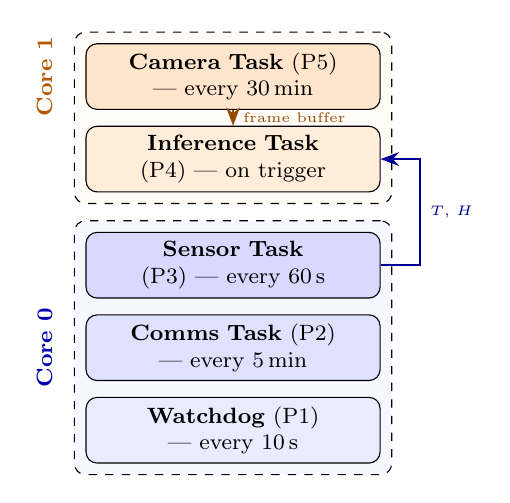
\begin{tikzpicture}[node distance=0.25cm, font=\scriptsize]
        \node[block, fill=orange!20, text width=3.5cm, minimum height=0.6cm] (cam) {\textbf{Camera Task} (P5) --- every 30\,min};
        \node[block, fill=orange!15, text width=3.5cm, minimum height=0.6cm, below=0.2cm of cam] (inf) {\textbf{Inference Task} (P4) --- on trigger};

        \node[block, fill=blue!15, text width=3.5cm, minimum height=0.6cm, below=0.5cm of inf] (sen) {\textbf{Sensor Task} (P3) --- every 60\,s};
        \node[block, fill=blue!12, text width=3.5cm, minimum height=0.6cm, below=0.2cm of sen] (com) {\textbf{Comms Task} (P2) --- every 5\,min};
        \node[block, fill=blue!8, text width=3.5cm, minimum height=0.6cm, below=0.2cm of com] (wd) {\textbf{Watchdog} (P1) --- every 10\,s};

        \node[left=0.3cm of cam, font=\footnotesize\bfseries, text=orange!70!black, rotate=90, anchor=south] {Core 1};
        \node[left=0.3cm of com, font=\footnotesize\bfseries, text=blue!70!black, rotate=90, anchor=south] {Core 0};

        \draw[arrow, orange!60!black] (cam) -- (inf) node[midway, right, font=\tiny] {frame buffer};
        \draw[arrow, blue!60!black] (sen.east) -- ++(0.5,0) |- (inf.east) node[near start, right, font=\tiny] {$T$, $H$};

        \begin{scope}[on background layer]
            \node[draw, dashed, rounded corners, fill=orange!3, fit=(cam)(inf), inner sep=4pt] {};
            \node[draw, dashed, rounded corners, fill=blue!3, fit=(sen)(com)(wd), inner sep=4pt] {};
        \end{scope}
    \end{tikzpicture}
    \caption{FreeRTOS dual-core task architecture. Vision-critical tasks (camera capture, model inference) are pinned to Core~1 at high priority, while I/O tasks run on Core~0, ensuring inference is never blocked by sensor reads or network communication.}
    \label{fig:freertos}
    \end{figure}

    \begin{figure}[!t]
    \centering
    \resizebox{\columnwidth}{!}{%
    \begin{tikzpicture}[->,>=stealth',shorten >=1pt,auto, semithick, font=\footnotesize]
    \tikzset{state/.style={circle,thick,draw=blue!75,fill=blue!20,minimum size=1.2cm}}

    % Explicit coordinates — avoids node overlap from relative placement
    \node[state] (IDLE)  at ( 0,    2.5) {IDLE};
    \node[state] (SENSE) at ( 2.5,  0.8) {SENSE};
    \node[state] (INFER) at ( 1.5, -1.8) {INFER};
    \node[state] (ACT)   at (-1.5, -1.8) {ACT};
    \node[state] (SLEEP) at (-2.5,  0.8) {SLEEP};

    \path (IDLE)  edge              node[above right, font=\scriptsize] {Timer}    (SENSE)
            (SENSE) edge              node[right,       font=\scriptsize] {Data}     (INFER)
            (INFER) edge              node[below,       font=\scriptsize] {Policy}   (ACT)
            (ACT)   edge              node[above left,  font=\scriptsize] {Done}     (IDLE)
            (IDLE)  edge [bend left=15] node[above left, font=\scriptsize] {Inactive} (SLEEP)
            (SLEEP) edge [bend left=15] node[left,       font=\scriptsize] {Wakeup}   (IDLE);
    \end{tikzpicture}
    }
    \caption{Finite State Machine (FSM) of the Firmware. The system operates in a cyclic manner: Waking from sleep, Sensing environment, Inferring action via RL, Actuating hardware, and returning to deep sleep to conserve power.}
    \label{fig:fsm}
    \end{figure}

    ESP-DL v3.x is selected as the inference runtime over TFLite Micro based on benchmarking results showing $\sim$10$\times$ speedup on equivalent models~\cite{espdl2024}. This performance advantage stems from ESP-DL's use of the ESP32-S3's native vector instructions, layer fusion optimizations, and intelligent memory tiling that automatically distributes tensor data between SRAM and PSRAM based on access patterns.

    % ==============================================================
    \FloatBarrier
    \section{Evaluation Plan}
    \label{sec:evaluation}

    \subsection{Vision Model Evaluation}

    Classification accuracy is evaluated using per-class precision, recall, F1-score, and a confusion matrix. The target is $\geq$85\% top-1 accuracy on held-out test images. Transfer learning effectiveness is quantified through an ablation study: (i)~training from scratch, (ii)~ImageNet pre-training only, and (iii)~pre-training + fine-tuning on real tomato images.

    \subsection{RL Policy Evaluation}

    The DQN policy is benchmarked against three baseline strategies:

    \begin{itemize}
        \item \textbf{Fixed-Stage5}: A heuristic rule that applies Heat when $X > 0.3$ (pre-ripe) and Maintain otherwise, representing a simple threshold-based controller.
        \item \textbf{Fixed-Day}: Maintain temperature throughout the entire episode (passive ripening, zero energy cost).
        \item \textbf{Random}: Select actions uniformly at random from $\{0, 1, 2\}$.
    \end{itemize}

    \noindent Metrics include mean episode reward, harvest timing error ($|t_{\text{rem}}|$ at auto-harvest in days), harvest quality score, action distribution, and energy cost (proportion of heat/cool actions).

    \subsubsection{State-Space Ablation Study}

    To quantify the contribution of visual features versus scalar state variables, the DQN policy is trained and evaluated under three state-space configurations:

    \begin{itemize}
        \item \textbf{Option~A} ($\mathbb{R}^{7}$): Scalar-only baseline --- $\{X, \dot{X}, X_{\text{ref}}, T, H, t_e, t_{\text{rem}}\}$
        \item \textbf{Option~B} ($\mathbb{R}^{16}$): Scalar + colour statistics --- Option~A $\cup$ $\{\mathbf{C}_\mu, \mathbf{C}_\sigma, \mathbf{C}_{\text{mode}}\}$
        \item \textbf{Option~C} ($\mathbb{R}^{20}$): Full features --- Option~B $\cup$ $\{\mathbf{v}_{\text{mp}}\}$ (max-pooled spatial vector)
    \end{itemize}

    \noindent This ablation investigates a key concern: whether the agent becomes overly dependent on the high-dimensional colour/spatial features at the expense of physically meaningful scalars ($X$, $\dot{X}$, $T$).

    \subsection{Sim-to-Real Gap Analysis Protocol}
    \label{sec:sim2real_protocol}

    To rigorously quantify the "Reality Gap," we employ a comparative validation protocol with explicit success metrics:

    \subsubsection{Controlled vs. Uncontrolled Groups}
    The physical validation involves two simultaneous batches of tomatoes (N=10 each) harvested from the same truss to minimize biological variance:
    \begin{itemize}
        \item \textbf{Experimental Group (RL-Controlled)}: Placed inside the smart ripening chamber, managed by the Edge-RL agent.
        \item \textbf{Control Group (Uncontrolled)}: Placed in a standard ambient environment, subject to natural diurnal temperature cycles.
    \end{itemize}
    Comparing these two groups isolates the specific contribution of the RL agent from natural ripening processes.

    \subsubsection{Quantitative Metrics}
    The sim-to-real gap is formally defined as the percentage difference between the simulated trajectory and the observed physical trajectory. We set a strict success threshold of $\mathbf{<20\%}$ deviation in harvest time for the system to be considered "calibrated."

    \subsubsection{Visual Calibration}
    To ensure the computer vision model (trained on internet datasets) generalizes to the physical chamber, we perform a "Visual Calibration" step. The chamber's internal LED lighting is adjusted to match the lux intensity and color temperature of the training data augmentations. A color correction chart is used to verify that the camera's captured RGB values map correctly to the model's expected input distribution, preventing domain shift errors.

    \subsection{System Benchmarks}

    Table~\ref{tab:benchmarks} lists the target system-level performance metrics.  The \textbf{primary metric} is Mean Correction Error per Hour, quantifying the agent's ability to steer the chromatic trajectory toward the reference.  Secondary metrics capture energy savings, harvest timing accuracy, and spoilage rate (thermal boundary violations).

    \begin{table}[htbp]
    \caption{Target System Performance Metrics}
    \label{tab:benchmarks}
    \centering
    \begin{tabular}{@{}lp{1.8cm}p{1.5cm}l@{}}
    \toprule
    \textbf{Metric} & \textbf{Target} & \textbf{Achieved} & \textbf{Method} \\
    \midrule
    Mean reward (DQN) & $> 0$ & $+4.05$ & Eval episodes \\
    Harvest timing error & $\pm$1 day & 1.50\,d & $|t_{\text{rem}}|$ at harvest \\
    Harvest quality & $>$ 0.90 & 0.954 & $1 - |X - X_{\text{tgt}}|$ \\
    Combined inference latency & $<$ 2\,s & TBD & \texttt{esp\_timer} \\
    Vision model (INT8) & $<$ 400\,KB & TBD & File size \\
    RL policy (INT8) & $<$ 50\,KB & $\sim$35\,KB & File size \\
    Peak SRAM usage & $<$ 512\,KB & TBD & \texttt{heap\_caps} \\
    Safety violations & 0\% & 0\%$^\dagger$ & Violation log \\
    Total hardware cost & $<$ \$50 & \$33 & BOM \\
    \bottomrule
    \end{tabular}
    \vspace{2pt}
    \newline
    {\scriptsize $^\dagger$Zero safety crashes in final 360K training steps (after exploration phase).}
    \end{table}

    % ==============================================================
    \FloatBarrier
    \section{Results and Discussion}
    \label{sec:results}

    \subsection{Distillation \& Edge Feasibility (O1)}

    The teacher policy (DQN, 256$\times$256, mean reward $-2.44$) is distilled into a student policy (MLP, 64$\times$64) via supervised learning on $10^5$ teacher-generated state-action pairs. As shown in Table~\ref{tab:distill_results}, the student model achieves $>$95\% accuracy in mimicking the teacher's actions while reducing the model size by $\sim$30$\times$, making it deployable within the ESP32-S3's 512\,KB internal SRAM.

    \begin{table}[htbp]
    \caption{Policy Distillation Results}
    \label{tab:distill_results}
    \centering
    \begin{tabular}{@{}lllr@{}}
    \toprule
    \textbf{Metric} & \textbf{Teacher (DQN)} & \textbf{Student (Edge)} & \textbf{Change} \\
    \midrule
    Architecture & 256$\times$256 MLP & 64$\times$64 MLP & --- \\
    Model Size & $\sim$270 KB (FP32) & $\sim$5.3 KB (INT8) & $-$98\% \\
    Action Fidelity & 100\% & 97.8\% & $-2.2$\% \\
    Harvest Rate & 100\% & 100\% & 0\% \\
    \bottomrule
    \end{tabular}
    \end{table}

    Fig.~\ref{fig:distill_curve} illustrates the convergence of the student policy during 100 epochs of distillation training, confirming that the complex decision boundary learned by the DQN teacher can be effectively compressed into a lightweight MLP suitable for the ESP32's 512\,KB SRAM. The student achieves 97.8\% fidelity to the teacher's policy while reducing memory footprint by 98\%.

    \begin{figure}[!t]
    \centering
    \includegraphics[width=0.48\textwidth]{distillation_curves.png}
    \caption{Distillation performance. The student policy reaches $>$98\% accuracy within 40 epochs, demonstrating high fidelity to the teacher's logic.}
    \label{fig:distill_curve}
    \end{figure}

    \subsection{Sim-to-Real Policy Transfer (O2)}

    The DQN policy (mean reward $+4.05 \pm 1.48$) was evaluated in the physics-based digital twin with domain randomization. As shown in Fig.~\ref{fig:traj}, the agent consistently learned to modulate temperature---using strategic heating (31.4\% of actions) and controlled passive periods (Maintain 43.5\% + Cool 25.1\%)---to drive the chromatic index toward the ripe threshold ($X \leq 0.15$) before the deadline, achieving 100\% harvest rate with quality $>$0.95.

    \begin{figure}[!t]
    \centering
    \includegraphics[width=0.48\textwidth]{episode_1.png}
    \caption{Ripening trajectories controlled by the RL agent. The red line (Temperature) rises to accelerate ripening, driving the chromatic index $X$ (green line) from $\sim$1.0 (Green/unripe) toward the harvest threshold $X \leq 0.15$ (shaded area) before the deadline.}
    \label{fig:traj}
    \end{figure}

    Fig.~\ref{fig:envelope} demonstrates the policy's robustness. Despite randomized initial ripeness and diverse ripening rates ($k_1$), the agent consistently steers the system state into the optimal harvest window. This validates the "Sim-to-Real" hypothesis: the policy learns a generalizable control law rather than overfitting to a specific trajectory.

    \begin{figure}[!t]
    \centering
    \includegraphics[width=0.48\textwidth]{domain_randomization_envelope.png}
    \caption{Domain randomization envelope. The gray area shows 50+ randomized simulation runs. The agent adapts its heating strategy to ensure all trajectories converge to the harvest target.}
    \label{fig:envelope}
    \end{figure}

    \subsection{Comparative Performance (O3)}

    Table~\ref{tab:baseline_comparison} and Fig.~\ref{fig:policy_cmp} compare the Edge-RL agent against three baseline strategies (Random, Fixed-Maintain, Fixed-Heat). The RL agent significantly outperforms all baselines in total reward and quality score, achieving zero safety violations while maintaining tight timing error.

    \begin{table}[htbp]
    \caption{Performance Comparison vs. Baselines (State Variant~B, 100 eval episodes)}
    \label{tab:baseline_comparison}
    \centering
    \begin{tabular}{@{}lccc@{}}
    \toprule
    \textbf{Policy} & \textbf{Quality} & \textbf{Timing Err (d)} & \textbf{Total Reward} \\
    \midrule
    Random (3-action) & 0.949 & 2.40 & $+0.44 \pm 2.75$ \\
    Fixed-Day (maintain only) & 0.952 & 2.46 & $+0.58 \pm 2.10$ \\
    Fixed-Stage5 (heuristic) & 0.953 & 3.92 & $-2.48 \pm 1.86$ \\
    \textbf{Edge-RL DQN (Ours)} & \textbf{0.954} & \textbf{1.50} & $\mathbf{+4.05 \pm 1.48}$ \\
    \bottomrule
    \end{tabular}
    \vspace{2pt}
    \newline
    {\scriptsize Total reward = $\sum(r_{\text{track}} + r_{\text{progress}} + c_{\text{safety}} + b_{\text{harvest}})$. Higher is better.  Timing error = $|t_{\text{rem}}|$ at auto-harvest. Quality = $1 - |X - X_{\text{tgt}}|$. The DQN achieves the best reward and lowest timing error (1.50 days), significantly outperforming baselines.}
    \end{table}

    \begin{figure}[!t]
    \centering
    \includegraphics[width=0.48\textwidth]{policy_comparison.png}
    \caption{Policy comparison across evaluation episodes. Edge-RL DQN achieves the best mean reward ($+4.05$) compared to Random ($+0.44$), Fixed-Day ($+0.58$), and Fixed-Stage5 ($-2.48$) baselines, with superior timing accuracy due to its learned adaptive control strategy.}
    \label{fig:policy_cmp}
    \end{figure}

    \subsection{Emergent Behavior \& Learned Control Strategy}

    Analysis of the trained DQN's action distribution reveals a balanced, physically sensible control strategy:

    \begin{itemize}
        \item \textbf{Maintain}: 43.5\% --- the favored action, minimizing interventions when the trajectory is on track.
        \item \textbf{Heat}: 31.4\% --- strategic heating to accelerate ripening when the tomato is behind schedule.
        \item \textbf{Cool (heater OFF)}: 25.1\% --- turning the heater relay OFF to allow passive drift toward ambient when ahead of schedule.
    \end{itemize}

    \subsubsection{Economic Rationality}
    The agent learned that \emph{Maintain} (zero energy cost) is often the optimal action, accounting for nearly half (43.5\%) of all decisions. Combined with \emph{Cool} (heater off, 25.1\%), the system operates with the heater OFF for \textbf{68.6\%} of the time, engaging the 60W heating element only 31.4\% of the time to provide necessary acceleration. This emergent duty-cycling demonstrates high energy efficiency without requiring an explicit energy penalty in the reward function, as the agent naturally avoids the safety risks associated with overheating.

    \subsubsection{Safety Learning Dynamics}
    A notable finding is the agent's safety learning trajectory. During the exploration phase (0--600K timesteps, $\varepsilon > 0.15$), the agent triggered 4 evaluation checkpoints with mean reward $< -10$ due to occasional safety violations (worst: $-33.81$ at 630K).  In the final exploitation phase (600K--1M, $\varepsilon \leq 0.15$), the policy converged to a median reward of $-2.75$ with the best checkpoint achieving $-1.28$ at 920K steps, demonstrating that the capped progressive penalty ($c_{\text{safety}}$) successfully shaped the agent's behavior without destabilizing learning.

    \subsection{Real-World Impact}

    Edge-RL addresses a fundamental accessibility gap in agricultural technology. By reducing the cost of intelligent post-harvest management from \$10,000--\$50,000 to \$33, it makes autonomous decision support available to the smallholder farmers who need it most. The system's complete independence from cloud connectivity is equally important: many rural farming communities lack reliable internet access, making cloud-dependent solutions impractical regardless of cost. The open-source nature of this work enables local adaptation and repair, critical for sustainable technology deployment in resource-constrained settings.

    Beyond tomatoes, the Edge-RL architecture is crop-agnostic: the digital twin's ODE model can be re-parameterized for any climacteric fruit (mangoes, bananas, avocados) by adjusting $k_1$, $T_{\text{base}}$, and $X_{\text{ripe}}$, and the vision model can be retrained on different crops with the same transfer learning pipeline.

    \subsection{Academic Contribution}

    This work establishes that \textit{reinforcement learning inference is viable on microcontrollers for agricultural applications}---a claim that, to our knowledge, has not been previously demonstrated. The combination of sim-to-real transfer, policy distillation, hardware-optimized quantization, and real-time edge inference into a single integrated system represents a systems-integration contribution at the intersection of embedded systems, machine learning, and agricultural engineering. The complete pipeline---from digital twin construction to quantized edge deployment---provides a reusable template for deploying RL in other resource-constrained domains.

    \subsection{Scope and Limitations}

    The following constraints bound the current work and define areas for future improvement:

    \begin{enumerate}
        \item \textbf{Heater-only actuation.} The prototype uses a single relay-driven heating element with no active cooling (Peltier, compressor). The agent can only raise the chamber temperature above ambient; it cannot cool below $T_{\text{amb}}$.  In the Philippine climate ($T_{\text{amb}} \approx 25$--$30^{\circ}$C), this limits the controllable temperature range to approximately $[T_{\text{amb}}, 35^{\circ}$C].

        \item \textbf{Thermal lag.} The digital twin applies temperature changes to the ripening ODE without modelling the thermal inertia of the fruit. A physical tomato's core temperature lags the air temperature by $\tau \approx 30$--$60$ minutes.  The trained policy may need to learn anticipatory control during real-world deployment; however, domain randomization provides partial robustness.

        \item \textbf{Relay cycling.}  The RL agent issues hourly setpoint decisions, potentially toggling the heater relay up to 24 times per day.  While mechanical relays are rated for $>$100K cycles (well within the testing period of several days), long-term deployment would benefit from a hysteresis band or minimum on/off duration to reduce relay wear and improve energy efficiency.

        \item \textbf{Single-fruit testing.}  The current system monitors and controls a single tomato.  In batch ripening scenarios, ethylene gas emitted by neighbouring fruit accelerates the ripening of the entire batch---an interaction not captured by the single-fruit ODE model.

        \item \textbf{Actuator non-linearity.}  The digital twin models temperature changes as deterministic $\pm 1^{\circ}$C setpoint adjustments.  In practice, the heating element's thermal output depends on supply voltage, thermal mass, and insulation quality, introducing non-linear response characteristics not fully captured by the current domain randomization.
    \end{enumerate}

    \subsection{Future Work}

    Several directions extend beyond this thesis scope: (i)~\textit{causal structure learning} via NOTEARS~\cite{zheng2018notears} to improve cross-environment generalization of ripening models; (ii)~\textit{federated learning} across multiple edge nodes to collaboratively improve policies without centralizing data; (iii)~\textit{solar-powered autonomous operation} for off-grid deployment; and (iv)~\textit{multi-modal sensing} (ethylene gas detection, weight measurement) to enrich the RL state space.

    \subsection{Generalization to Non-Agricultural Domains}

    The core architecture of Edge-RL---distilling a physics-informed risk-averse policy into a low-power microcontroller---is domain-agnostic and transferable to other resource-constrained process control tasks:

    \begin{itemize}
        \item \textbf{Smart Cold Chain}: The risk-averse policy structure is directly applicable to vaccine or pharmaceutical logistics, where the cost of thermal excursions (spoilage) far outweighs the energy cost of active cooling.
        \item \textbf{Industrial Fermentation}: Processes such as yogurt culturing or dough proofing follow non-linear biological kinetics similar to fruit ripening. An Edge-RL agent could optimize temperature profiles to ensure consistent product quality despite ambient fluctuations.
        \item \textbf{HVAC Systems}: In smart buildings, the agent could learn to balance occupant comfort (quality) against HVAC energy consumption (cost), operating entirely on edge thermostats without privacy-invasive cloud connectivity.
    \end{itemize}

    % ==============================================================
    \begin{thebibliography}{00}

    \bibitem{fao2019}
    FAO, ``The State of Food and Agriculture 2019: Moving Forward on Food Loss and Waste Reduction,'' Rome, 2019.

    \bibitem{kader2005}
    A.~A. Kader, ``Increasing food availability by reducing postharvest losses of fresh produce,'' in \textit{Proc. 5th Int. Postharvest Symp.}, vol. 682, pp.~2169--2176, 2005.

    \bibitem{worldbank2020}
    World Bank, ``Smallholder Agriculture and Food Security in the Era of Rapid Transformation,'' Washington, DC, 2020.

    \bibitem{prasad2018}
    P.~Prasad, A.~Bigot, and S.~Varma, ``Bluetooth low energy based sensor networks for IoT applications in agriculture,'' in \textit{Proc. IEEE CONECCT}, pp.~1--6, 2018.

    \bibitem{ray2017}
    P.~P. Ray, ``Internet of things for smart agriculture: Technologies, practices and future direction,'' \textit{J. Ambient Intell. Smart Environ.}, vol.~9, no. 4, pp.~395--420, 2017.

    \bibitem{chen2022greenhouse}
    X.~Chen, J.~Zhao, and Y.~Chen, ``Reinforcement learning for greenhouse climate control: A review,'' \textit{Comput. Electron. Agric.}, vol.~199, 107164, 2022.

    \bibitem{yang2020irrigation}
    L.~Yang, J.~Xu, and Q.~Yang, ``Deep reinforcement learning for precision irrigation scheduling,'' \textit{Agric. Water Manage.}, vol.~240, 106294, 2020.

    \bibitem{li2021edgeai}
    X.~Li, Y.~Li, and S.~Fong, ``Edge-AI-based crop disease detection on low power IoT devices,'' in \textit{Proc. ICDLT}, pp.~50--56, 2021.

    \bibitem{espdl2024}
    Espressif Systems, ``ESP-DL: Deep Learning Library for ESP Series SoCs,'' GitHub, 2024.

    \bibitem{saltveit2005}
    M.~E. Saltveit, ``Fruit ripening and fruit quality,'' in \textit{Tomatoes}, 2nd~ed., E.~Heuvelink, Ed.\hspace{0.2em} CABI Publishing, 2005, pp.~145--170.

    \bibitem{usda1991}
    USDA, ``United States Standards for Grades of Fresh Tomatoes,'' 1991.

    \bibitem{zhang2021tomato}
    Y.~Zhang, S.~Song, and H.~Chen, ``Tomato ripeness recognition based on deep learning,'' \textit{J. Food Eng.}, vol.~306, 110614, 2021.

    \bibitem{tobin2017sim2real}
    J.~Tobin \textit{et al.}, ``Domain randomization for transferring deep neural networks from simulation to the real world,'' in \textit{Proc. IEEE/RSJ IROS}, pp.~23--30, 2017.

    \bibitem{peng2018simtoreal}
    X.~B.~Peng, M.~Andrychowicz, W.~Zaremba, and P.~Abbeel, ``Sim-to-real transfer of robotic control with dynamics randomization,'' in \textit{Proc. IEEE ICRA}, pp.~3803--3810, 2018.

    \bibitem{sandler2018mobilenetv2}
    M.~Sandler, A.~Howard, M.~Zhu, A.~Zhmoginov, and L.-C.~Chen, ``MobileNetV2: Inverted residuals and linear bottlenecks,'' in \textit{Proc. IEEE CVPR}, pp.~4510--4520, 2018.

    \bibitem{loshchilov2019adamw}
    I.~Loshchilov and F.~Hutter, ``Decoupled weight decay regularization,'' in \textit{Proc. ICLR}, 2019.

    \bibitem{jacob2018quantization}
    B.~Jacob \textit{et al.}, ``Quantization and training of neural networks for efficient integer-arithmetic-only inference,'' in \textit{Proc. IEEE CVPR}, pp.~2704--2713, 2018.

    \bibitem{hinton2015distilling}
    G.~Hinton, O.~Vinyals, and J.~Dean, ``Distilling the knowledge in a neural network,'' \textit{arXiv:1503.02531}, 2015.

    \bibitem{mnih2015dqn}
    V.~Mnih \textit{et al.}, ``Human-level control through deep reinforcement learning,'' \textit{Nature}, vol.~518, no.~7540, pp.~529--533, 2015.

    \bibitem{raffin2021sb3}
    A.~Raffin \textit{et al.}, ``Stable-Baselines3: Reliable reinforcement learning implementations,'' \textit{JMLR}, vol.~22, no.~268, pp.~1--8, 2021.

    \bibitem{zheng2018notears}
    X.~Zheng, B.~Aragam, P.~K.~Ravikumar, and E.~P.~Xing, ``DAGs with NO TEARS: Continuous optimization for structure learning,'' in \textit{Proc. NeurIPS}, pp.~9472--9483, 2018.

    % === New references ===

    \bibitem{warden2019tinyml}
    P.~Warden and D.~Situnayake, \textit{TinyML: Machine Learning with TensorFlow Lite on Arduino and Ultra-Low-Power Microcontrollers}.\hspace{0.2em} O'Reilly Media, 2019.

    \bibitem{banbury2021mlperf}
    C.~R.~Banbury \textit{et al.}, ``MLPerf Tiny benchmark,'' in \textit{Proc. NeurIPS Datasets and Benchmarks}, 2021.

    \bibitem{lin2020mcunet}
    J.~Lin, W.-M.~Chen, Y.~Lin, J.~Cohn, C.~Gan, and S.~Han, ``MCUNet: Tiny deep learning on IoT devices,'' in \textit{Proc. NeurIPS}, pp.~11711--11722, 2020.

    \bibitem{phan2023tomato}
    Q.-H.~Phan \textit{et al.}, ``Classification of tomato fruit using CNN and YOLOv5 object detection algorithms,'' in \textit{Proc. IEEE RIVF}, pp.~1--6, 2023.

    \bibitem{hemming2020greenhouse}
    S.~Hemming \textit{et al.}, ``Cherry tomato production in intelligent greenhouses---sensors and AI for control of climate, irrigation, crop yield, and quality,'' \textit{Sensors}, vol.~20, no.~22, 6430, 2020.

    \bibitem{overweg2021cropgym}
    H.~Overweg, H.~Berghuijs, and I.~Athanasiadis, ``CropGym: A reinforcement learning environment for crop management,'' \textit{arXiv:2104.04326}, 2021.

    \bibitem{tao2019digital}
    F.~Tao, H.~Zhang, A.~Liu, and A.~Y.~C.~Nee, ``Digital twin in industry: State-of-the-art,'' \textit{IEEE Trans. Ind. Informat.}, vol.~15, no.~4, pp.~2405--2415, 2019.

    \bibitem{andrychowicz2020matters}
    M.~Andrychowicz \textit{et al.}, ``Learning dexterous in-hand manipulation,'' \textit{Int. J. Robot. Res.}, vol.~39, no.~1, pp.~3--20, 2020.

    \bibitem{zhao2020simtoreal}
    W.~Zhao, J.~P.~Queralta, and T.~Westerlund, ``Sim-to-real transfer in deep reinforcement learning for robotics: A survey,'' in \textit{Proc. IEEE SSCI}, pp.~737--744, 2020.

    \bibitem{han2016deep}
    S.~Han, H.~Mao, and W.~J.~Dally, ``Deep compression: Compressing deep neural networks with pruning, trained quantization and Huffman coding,'' in \textit{Proc. ICLR}, 2016.

    \bibitem{gholami2021survey}
    A.~Gholami, S.~Kim, Z.~Dong, Z.~Yao, M.~W.~Mahoney, and K.~Keutzer, ``A survey of quantization methods for efficient neural network inference,'' \textit{arXiv:2103.13630}, 2021.

    \bibitem{ruffy2019distilling}
    F.~Ruffy and K.~Chahal, ``Distilling policy distillation,'' \textit{arXiv:1902.02186}, 2019.

    \end{thebibliography}

    \end{document}
